\documentclass{standalone}
\usepackage{tikz}
\usetikzlibrary{patterns, positioning}


\begin{document}
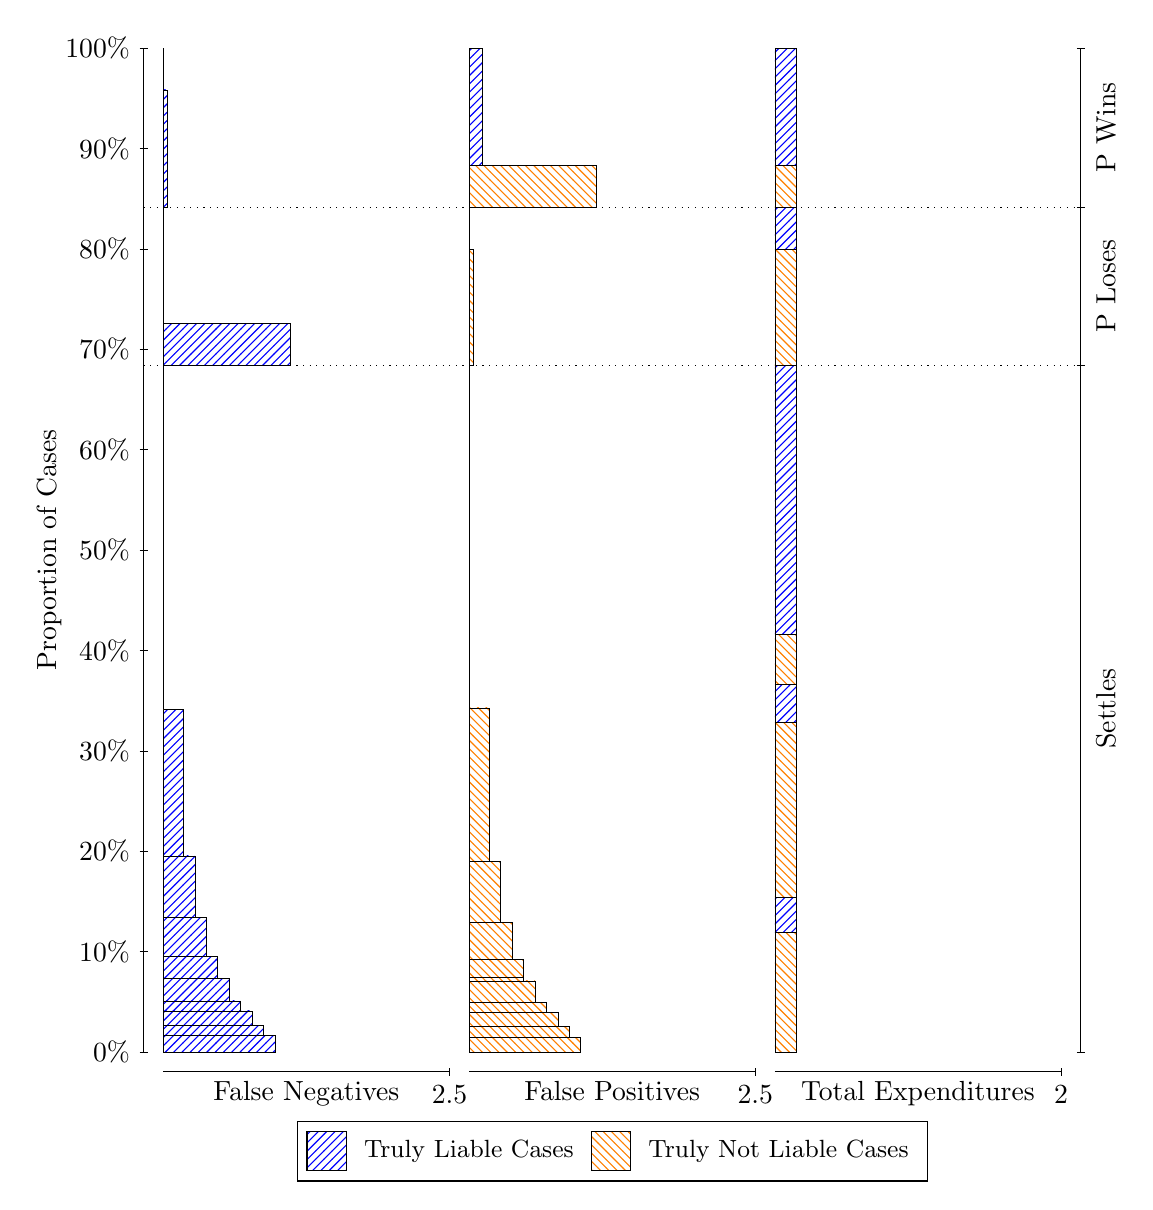
\begin{tikzpicture}
\draw[black, very thin] (1.5,1.75) -- (1.5,14.5);
\node[rotate=90, text=black, anchor=center] at (0.3, 8.125) {Proportion of Cases};
\draw[black, very thin] (1.45,1.75) -- (1.55,1.75);
\node[text=black, anchor=east] at (1.45, 1.75) {0\%};
\draw[black, very thin] (1.45,3.025) -- (1.55,3.025);
\node[text=black, anchor=east] at (1.45, 3.025) {10\%};
\draw[black, very thin] (1.45,4.3) -- (1.55,4.3);
\node[text=black, anchor=east] at (1.45, 4.3) {20\%};
\draw[black, very thin] (1.45,5.575) -- (1.55,5.575);
\node[text=black, anchor=east] at (1.45, 5.575) {30\%};
\draw[black, very thin] (1.45,6.85) -- (1.55,6.85);
\node[text=black, anchor=east] at (1.45, 6.85) {40\%};
\draw[black, very thin] (1.45,8.125) -- (1.55,8.125);
\node[text=black, anchor=east] at (1.45, 8.125) {50\%};
\draw[black, very thin] (1.45,9.4) -- (1.55,9.4);
\node[text=black, anchor=east] at (1.45, 9.4) {60\%};
\draw[black, very thin] (1.45,10.675) -- (1.55,10.675);
\node[text=black, anchor=east] at (1.45, 10.675) {70\%};
\draw[black, very thin] (1.45,11.95) -- (1.55,11.95);
\node[text=black, anchor=east] at (1.45, 11.95) {80\%};
\draw[black, very thin] (1.45,13.225) -- (1.55,13.225);
\node[text=black, anchor=east] at (1.45, 13.225) {90\%};
\draw[black, very thin] (1.45,14.5) -- (1.55,14.5);
\node[text=black, anchor=east] at (1.45, 14.5) {100\%};

\draw[black, very thin] (13.4,1.75) -- (13.4,14.5);
\draw[black, very thin] (13.35,1.75) -- (13.45,1.75);
\node[anchor=west] at (13.35, 1.75) {};
\draw[black, very thin] (13.35,10.472) -- (13.45,10.472);
\node[anchor=west] at (13.35, 10.472) {};
\draw[black, very thin] (13.35,12.476) -- (13.45,12.476);
\node[anchor=west] at (13.35, 12.476) {};
\draw[black, very thin] (13.35,14.5) -- (13.45,14.5);
\node[anchor=west] at (13.35, 14.5) {};

\draw[black, very thin, pattern color=blue, pattern=north east lines] (1.75,1.75) rectangle (3.167,1.9559);
\draw[black, very thin, pattern color=blue, pattern=north east lines] (1.75,1.9559) rectangle (3.0217,2.0923);
\draw[black, very thin, pattern color=blue, pattern=north east lines] (1.75,2.0923) rectangle (2.8763,2.2713);
\draw[black, very thin, pattern color=blue, pattern=north east lines] (1.75,2.2713) rectangle (2.731,2.3986);
\draw[black, very thin, pattern color=blue, pattern=north east lines] (1.75,2.3986) rectangle (2.5857,2.6801);
\draw[black, very thin, pattern color=blue, pattern=north east lines] (1.75,2.6801) rectangle (2.4403,2.9607);
\draw[black, very thin, pattern color=blue, pattern=north east lines] (1.75,2.9607) rectangle (2.295,3.4579);
\draw[black, very thin, pattern color=blue, pattern=north east lines] (1.75,3.4579) rectangle (2.1497,4.2401);
\draw[black, very thin, pattern color=blue, pattern=north east lines] (1.75,4.2401) rectangle (2.0043,6.1012);
\draw[black, very thin, pattern color=orange, pattern=north west lines] (1.75,6.1012) rectangle (1.75,10.472);
\draw[black, very thin, pattern color=blue, pattern=north east lines] (1.75,10.472) rectangle (3.3668,11.004);
\draw[black, very thin, pattern color=orange, pattern=north west lines] (1.75,11.004) rectangle (1.75,12.476);
\draw[black, very thin, pattern color=blue, pattern=north east lines] (1.75,12.476) rectangle (1.8045,13.968);
\draw[black, very thin, pattern color=orange, pattern=north west lines] (1.75,13.968) rectangle (1.75,14.5);
\draw[black, very thin, pattern color=orange, pattern=north west lines] (5.6333,1.75) rectangle (7.0503,1.9402);
\draw[black, very thin, pattern color=orange, pattern=north west lines] (5.6333,1.9402) rectangle (6.905,2.0747);
\draw[black, very thin, pattern color=orange, pattern=north west lines] (5.6333,2.0747) rectangle (6.7597,2.2531);
\draw[black, very thin, pattern color=orange, pattern=north west lines] (5.6333,2.2531) rectangle (6.6143,2.3796);
\draw[black, very thin, pattern color=orange, pattern=north west lines] (5.6333,2.3796) rectangle (6.469,2.653);
\draw[black, very thin, pattern color=orange, pattern=north west lines] (5.6333,2.653) rectangle (6.3237,2.6942);
\draw[black, very thin, pattern color=orange, pattern=north west lines] (5.6333,2.6942) rectangle (6.3237,2.9237);
\draw[black, very thin, pattern color=orange, pattern=north west lines] (5.6333,2.9237) rectangle (6.1783,3.3992);
\draw[black, very thin, pattern color=orange, pattern=north west lines] (5.6333,3.3992) rectangle (6.033,4.1702);
\draw[black, very thin, pattern color=orange, pattern=north west lines] (5.6333,4.1702) rectangle (5.8877,6.1206);
\draw[black, very thin, pattern color=blue, pattern=north east lines] (5.6333,6.1206) rectangle (5.6333,10.472);
\draw[black, very thin, pattern color=orange, pattern=north west lines] (5.6333,10.472) rectangle (5.6878,11.944);
\draw[black, very thin, pattern color=blue, pattern=north east lines] (5.6333,11.944) rectangle (5.6333,12.476);
\draw[black, very thin, pattern color=orange, pattern=north west lines] (5.6333,12.476) rectangle (7.2502,13.008);
\draw[black, very thin, pattern color=blue, pattern=north east lines] (5.6333,13.008) rectangle (5.7968,14.5);
\draw[black, very thin, pattern color=orange, pattern=north west lines] (9.5167,1.75) rectangle (9.7892,3.2672);
\draw[black, very thin, pattern color=blue, pattern=north east lines] (9.5167,3.2672) rectangle (9.7892,3.7099);
\draw[black, very thin, pattern color=orange, pattern=north west lines] (9.5167,3.7099) rectangle (9.7892,5.9337);
\draw[black, very thin, pattern color=blue, pattern=north east lines] (9.5167,5.9337) rectangle (9.7892,6.4211);
\draw[black, very thin, pattern color=orange, pattern=north west lines] (9.5167,6.4211) rectangle (9.7892,7.0507);
\draw[black, very thin, pattern color=blue, pattern=north east lines] (9.5167,7.0507) rectangle (9.7892,10.472);
\draw[black, very thin, pattern color=orange, pattern=north west lines] (9.5167,10.472) rectangle (9.7892,11.944);
\draw[black, very thin, pattern color=blue, pattern=north east lines] (9.5167,11.944) rectangle (9.7892,12.476);
\draw[black, very thin, pattern color=orange, pattern=north west lines] (9.5167,12.476) rectangle (9.7892,13.008);
\draw[black, very thin, pattern color=blue, pattern=north east lines] (9.5167,13.008) rectangle (9.7892,14.5);
\draw[black, dotted] (1.5,10.472) -- (13.4,10.472);
\draw[black, dotted] (1.5,12.476) -- (13.4,12.476);
\draw[black, very thin] (1.75,1.5) -- (5.3833,1.5);
\node[text=black, anchor=north] at (3.5667, 1.5) {False Negatives};
\draw[black, very thin] (5.3833,1.45) -- (5.3833,1.55);
\node[text=black, anchor=north] at (5.3833, 1.45) {2.5};

\draw[black, very thin] (5.6333,1.5) -- (9.2667,1.5);
\node[text=black, anchor=north] at (7.45, 1.5) {False Positives};
\draw[black, very thin] (9.2667,1.45) -- (9.2667,1.55);
\node[text=black, anchor=north] at (9.2667, 1.45) {2.5};

\draw[black, very thin] (9.5167,1.5) -- (13.15,1.5);
\node[text=black, anchor=north] at (11.333, 1.5) {Total Expenditures};
\draw[black, very thin] (13.15,1.45) -- (13.15,1.55);
\node[text=black, anchor=north] at (13.15, 1.45) {2};

\node[text=black, centered, rotate=90] at (13.72, 6.1109) {Settles};
\node[text=black, centered, rotate=90] at (13.72, 11.474) {P Loses};
\node[text=black, centered, rotate=90] at (13.72, 13.488) {P Wins};

\draw (7.449999999999999,1.5) node[draw=none] (baseCoordinate) {};
\begin{scope}[align=center]
        \matrix[scale=0.5, draw=black, below=0.5cm of baseCoordinate, nodes={draw}, column sep=0.1cm]{
            \node[rectangle, draw, minimum width=0.5cm, minimum height=0.5cm, pattern color=blue, pattern=north east lines] {}; &
            \node[draw=none, font=\small, text=black] (B) {Truly Liable Cases}; &
            \node[rectangle, draw, minimum width=0.5cm, minimum height=0.5cm, pattern color=orange, pattern=north west lines] {}; &
            \node[draw=none, font=\small, text=black] (B) {Truly Not Liable Cases}; \\
            };
\end{scope}

\end{tikzpicture}
\end{document}